%%%%%%%%%%%%%%%%%%%%%%%%%%%%%%%%%%%%%%%%%%%%%%%%%%%%%%%%%%%%%%%%%%%%
%%%%%%%%%%%%%%%%%%%%%%%%%%%%%%%%%%%%%%%%%%%%%%%%%%%%%%%%%%%%%%%%%%%%
%%%%%%%%%%%%%%%%%%%%%%%%%%%%%%%%%%%%%%%%%%%%%%%%%%%%%%%%%%%%%%%%%%%%
%%%%%%%%%%%%%%%%%%%%%%%%%%%%%%%%%%%%%%%%%%%%%%%%%%%%%%%%%%%%%%%%%%%%
\chapter{Outils de modélisation}\label{c:omod}


% pourquoi on parle de SOC ? Parce qu'on souhaite représenter des objets audiovisuels, leur production, leur description et que ceci ne peut se faire sans une représentation du vocabulaire utilisé dans la production audiovisuelle. 

Dans le cadre de la production audiovisuelle collaborative, qui implique à la fois des amateurs et des professionnels, un des enjeux que nous avons noté (\ref{sec:scien}) est de rendre plus compréhensible l'échange d'informations entre contributeurs. 
D'une part, nous avons des practiciens professionnels utilisant un ou plusieurs vocabulaires métiers suffisamment définis pour que l'on puisse en faire des dictionnaires (\cite{Journot2008}; \cite{Pinel2008}). 
Ces personnes font usage de la langue d'une manière précise, régie par des conventions et portée par une conception de la production audiovisuelle et de ses objets, que l'on suppose stabilisée, au moins localement (au sein d'un même pays, d'une même école de pensée, organisation, équipe etc.).
Toutefois, on s'attend à des variations dans les usages de la langue, au même titre que l'on suppose qu'il existe des variations entre pratiques des gens du métiers.
Cependant, il semble qu'il s'agit seulement de variations et qu'il soit possible alors d'identifier les éléments communs et distincts.

D'autre part, les amateurs, quant à eux, n'ont pas le support de ces conventions travaillées au quotidien.
Ils sont, au mieux, des intermittents éclairés qui ont saisi le sens d'éléments de langage propres aux métiers (par des lectures, des rencontres, des formations etc.). 
Il faut donc supposer qu'il y a tout à expliquer à ces amateurs, plutôt que de parier sur leur compréhension innée des métiers de la production audiovisuelle.
En particulier s'il s'agit de demander du contenu à des amateurs sous la forme d'un script de tournage, il faudra alors trouver un moyen d'expliciter cette commande et d'expliquer ou d'assister sa réalisation. 

Ainsi, l'écart entre collaborateurs (qu'ils soient tous professionnels, ou un mélange d'amateurs et de professionnels) peut se situer sur différents niveaux : 
\begin{liste} 
	\item au niveau du vocabulaire métier, comme les mots utilisés dans le script pour désigner tel ou tel type de plan etc. 
	Dans le cas d'amateurs, il faut supposer que ces mots sont inconnus ou méconnus ; dans le cas de professionnels, on préfèrera expliciter le vocabulaire afin d'éviter toute confusion. 
	
	\item au niveau des connaissances et de la manière de conceptualiser le métier, le cycle de production et ses objets. 
	Là encore, un amateur ne connaît pas ou très peu les détails classiques des méthodes de production professionnelle. 
	De plus, la production audiovisuelle étant organisée en projets distincts, les méthodes peuvent fortement varier entre la production d'un documentaire et d'une émission de variétés. 
	Chaque genre, chaque équipe aura donc ses propres objets, ses propres méthodes qu'il faut alors expliciter aux autres professionnels pour s'assurer de leur collaboration. 

	\item sur le plan pratique, il faut également remarquer que les compétences peuvent également varier fortement entre métiers, suivant les genres de production audiovisuelle. 
	Ainsi, en plus d'expliciter les échanges d'informations, il serait également souhaitable de proposer une assistance aux collaborateurs amateurs ou professionnels pour s'assurer que le résultat produit correspond bien à l'attente initiale. 	
\end{liste}


Nous présentons dans une première section un exemple de commande de tournage qui illustre ces différents écarts en impliquant des communautés d'amateurs et de professionnels (\ref{sec:cdcf}). 
Ce scénario d'usage nous permet de préciser les besoins en modélisation exprimées précédemment (\ref{sec:prob}).
Notamment, il apparaît nécessaire de représenter à la fois la ou les conceptualisation(s), le(s) vocabulaire(s) utilisé(s) ainsi que les résultats attendus par les acteurs de la chaîne de production audiovisuelle. 
Ainsi, nous nous intéresserons à l'utilisation de divers Systèmes d'Organisations de Connaissances (SOC, \cite{Zacklad2010}) pour mettre en place un partage d'information normalisée. 
Après un retour sur les définitions principales que nous utiliserons, nous examinerons les langages, modèles et normes existants qui permettent de représenter des SOC (\ref{sec:defs}).
La distinction entre terminologie et ontologie nous nous permet de détailler le fonctionnement d'une méthode de construction d'ontologie différentielle (\ref{sec:construction}).
Enfin, nous présenterons les langages permettant de représenter ces SOCs (\ref{sec:mods}). 

%Dans une seconde partie, nous examinerons les modèles de l'audiovisuel existants.




%%%%%%%%%%%%%%%%%%%%%%%%%%%%%%%%%%%%%%%%%%%%%%%%%%%%%%%%%%%%%%%%%%%%
%%%%%%%%%%%%%%%%%%%%%%%%%%%%%%%%%%%%%%%%%%%%%%%%%%%%%%%%%%%%%%%%%%%%
\section{Cahier des charges fonctionnel (n)}\label{sec:cdcf}


%%%%%%%%%%%%%%%%%%%%%%%%%%%%%%%%%%%%%%%%%%%%%%%%%%%%%%%%%%%%%%%%%%%%
\subsection{Scénario de commande de tournage}\label{sec:scenar}
Considèrons comme cas d'étude une commande de tournage en vue de réaliser des reportages sur des évènements culturels de type concert ou opéra. 
Il met en jeu trois communautés en collaboration :

\begin{itemize}
	\item la RTBF (Radio Télévision Belge Francophone) établit des commandes de contenu dans un jargon métier propre. Son objectif est d'externaliser dès que possible la réalisation de la commande. Cela implique une compréhension commune sur le contenu à réaliser qui passe par un accord sur la manière de décrire la commande. 
	
	\item le contenu commandé est tourné soit par la VRT (Radio-Télévision Flamande) qui utilise un jargon différent de la RTBF, soit des amateurs qui ne connaissent pas les concepts de la réalisation audiovisuelle. Dans le premier cas, la conceptualisation est commune, seuls les termes changent. Dans le second cas, il s'agit d'expliquer et d'illustrer les concepts utilisés \\
\end{itemize}

Le développement d'une application d'assistant de tournage pour guider les amateurs paraît souhaitable pour amener le contenu filmé à un niveau de qualité exploitable. 
Il faut cependant faire la distinction entre les propositions de dépôt spontané de contenu (comme le pratique une chaîne d'information telle que BFM\footnote{La rubrique témoins BFM permet à un utilisateur de déposer des photos ou vidéos sur le site. 
Après modération, le contenu est diffusé et peut même faire l'objet d'une vente. Voir http$:$//temoins.bfmtv.com/}) et les appels à contribution où le professionnel passe commande auprès d'amateurs en détaillant ses exigences. 

Dans ce dernier cadre, on souhaite fournir un plan de tournage au caméraman afin de guider sa prise de vue. 
Le plan de tournage est construit à partir de recommandations rédigées par un réalisateur (position, cadrage, lumière, etc.) utilisant un vocabulaire métier. 
L'originalité de l'application est d'adapter l'information présentée au caméraman suivant ses capacités (amateur, professionnel) ou son employeur si c'est un professionnel travaillant dans une tierce organisation. 
On suppose ainsi que malgré quelques variations dans le vocabulaire utilisé, les professionnels de l'audiovisuel utilisent les mêmes concepts pour décrire le contenu. 
Par exemple, la notion de cadrage fait appel à des concepts de valeurs de plan indiquant la portion visible d'un personnage à l'écran (voir Figure \ref{img:intro:script}, page \pageref{img:intro:script}).
Un \textit{plan américain} indique ainsi que le personnage principal est cadré de la tête jusqu'au dessus des genoux. 
Le terme est utilisé en Europe en rappel à son emploi caractéristique dans les films américains des années 1910-1940, notamment dans les westerns où il permettait de montrer l'ensemble du pistolet à la ceinture des personnages\footnote{Roger Boussinot, l'Encyclopédie du Cinéma, Bordas.}. 
Ce cadrage est aussi appelé \textit{plan 3/4} et en anglais 3/4 shot, medium-long shot ou american shot pour traduire l'expression popularisée en Europe. 
Si le terme utilisé varie suivant le lieu et la littérature de référence, la définition de ce type de cadrage est sans équivoque. 

%=============
% \begin{figure}[htb]
% \centering
% 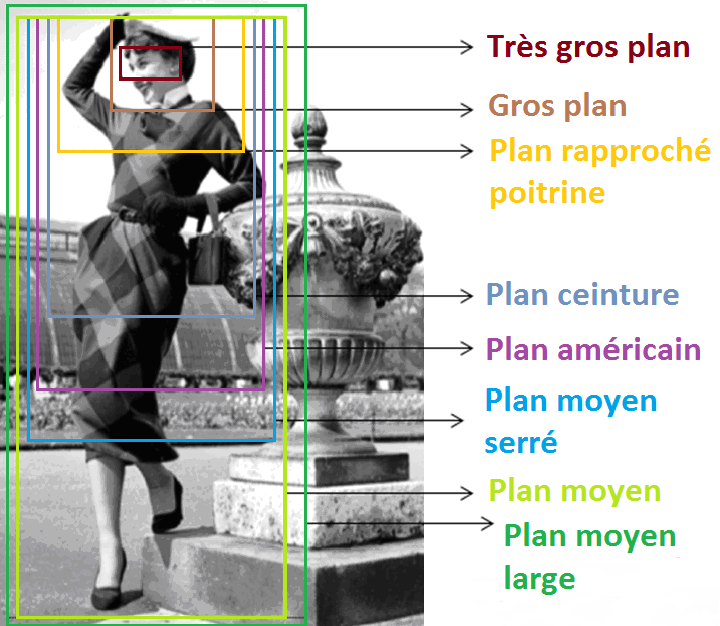
\includegraphics[width=0.5\textwidth]{./images/ValeurPlan-v1.png}
% \caption{Différentes valeurs de plan pour le cadrage d'un personnage à l'écran}
% \label{fig:cadrage}
% \end{figure}
%=============

Les amateurs quand à eux ignorent ces concepts et n'ont pas été initiés à ces pratiques. Ils ont donc besoin d'explications et d'illustrations pour comprendre les recommandations du réalisateur. 
Dans le cas du cadrage, une illustration graphique est d'autant plus pertinente. 
L'enjeu se situe donc dans la collaboration entre un prescripteur et un opérateur qui doivent s'accorder sur le contenu à produire malgré la différence de vocabulaire. 
% Un exemple des différences de présentation entre amateur et professionnel est illustré figure \ref{fig:prescription}.


% %%=============
% \begin{figure}[htb]
% \centering
% \includegraphics[width=0.3\textwidth]{./images/ShootingRecommandation-v1.png}
% \caption{Exemple de prescription de tournage à destination de professionnels (en haut) ou d'amateurs (en bas)}
% \label{fig:eda:prescription}
% \end{figure}
% %%=============


%%%%%%%%%%%%%%%%%%%%%%%%%%%%%%%%%%%%%%%%%%%%%%%%%%%%%%%%%%%%%%%%%%%%
\subsection{Besoins en modélisation}\label{sec:bm}
La mise en place d'une telle application nécessite de représenter le vocabulaire de la réalisation audiovisuelle dans toutes ses variations possibles et de le documenter suffisamment afin de le rendre compréhensible pour des novices. 
Cet objectif nous amène à considérer la construction d'une ressource termino-ontologique. L'ontologie permet de représenter les concepts partagés par les professionels de la réalisation audiovisuelle et la terminologie permet de capturer les différentes formes d'expression associées à ces concepts. 

La spécificité de notre problématique est de considérer la collaboration de communautés hétérogènes par leur degré de compréhension des concepts ou leur utilisation de la terminologie. 
Ceci nous amène à envisager la terminologie comme un moyen d'associer à des éléments ontologiques (concept, relation, instances) une chaîne lexicale ou des ressources média. 
Chaque chaîne ou ressource s'adresse en particulier à une communauté dont les membres partagent une capacité d'interprétation commune. 
Il n'existe donc plus une terminologie de référence par langue, mais des terminologies pour chaque communauté d'utilisateurs. 
On remarquera que notre acception de la terminologie sert bien à normaliser les pratiques linguistiques entre les membres d'une même organisation. 
En plus de cela, elle permet de fixer la manière de s'adresser à d'autres communautés.

Par ailleurs, les types de réalisations sont divers et nécessitent des concepts spécifiques pour être décrits. 
Une fiction se structure en séquences et en scènes alors que les documentaires ou magazines d'information se composent de sujets. 
La variabilité des types de contenu à filmer implique donc de pouvoir étendre le fond conceptuel initial pour représenter de nouveaux usages. 
De la même manière, la collaboration avec de nouveaux partenaires nécessite de pouvoir ajouter de nouvelles terminologies au fond conceptuel existant. 
Ontologie et terminologie doivent se gérer de manière indépendante. A partir de ces besoins, nous définissons maintenant les exigences en terme de modélisation. 

Nos besoins en modélisation peuvent être exprimés par les assertions suivantes:
\begin{enumerate}
	\item[(A1)] la variabilité des pratiques linguistiques des organisations et des communautés implique d'associer plusieurs termes à un même concept. 
	Il n'y a pas de choix des termes préférés par une communauté mais une \textit{correspondance} entre les termes d'une ou plusieurs communautés, quels que soient la langue et le code d'écriture utilisé.
	
	\item[(A2)] la variabilité de compréhension des communautés implique d'associer des explications (chaîne lexicale) ou des illustrations (ressource média) aux concepts afin d'en enrichir la \textit{documentation}. 
	
	\item[(A3)] la variabilité des cas de collaboration implique de pouvoir étendre la conceptualisation initiale ou la terminologie pour s'adapter à de nouvelles pratiques ou de nouvelles communautés. 
	Cela implique une gestion et une \textit{évolution} indépendante de l'ontologie et de la terminologie. 
\end{enumerate}


Dans le cas d'une demande de cadrage en plan américain, la demande est d'abord exprimée dans le jargon de la RTBF puis traduite dans le jargon de la VRT (plan américain pour la RTBF, plan 3/4 pour la VRT) [A1]. 
Ensuite, pour les amateurs, la terminologie est enrichie par des illustrations [A2]. Enfin, un nouveau concept de cadrage est ajouté (plan américain large ou plan moyen serré) [A3] en vue d'une nouvelle coopération avec la VRT. En plus de cela, le problème de la langue (français et flamand) s'ajoute à la question des jargons métiers. 
